\documentclass{article}

\usepackage{fancyhdr}
\usepackage{graphicx}  % This package allows the importing of images
\graphicspath{ {./} }
\usepackage[margin=1in]{geometry}
\usepackage{mdframed}
\usepackage{enumitem}
\usepackage{amsfonts}
\usepackage{graphicx}
\usepackage{commath}
\usepackage{amssymb}
\usepackage{outlines}
\usepackage[dvipsnames]{xcolor}
\usepackage{multicol}
\pagestyle{fancy}
\usepackage{hyperref}

\newcommand{\maketitletwo}{
    
    \rhead{Aditya Tapshalkar \\ YOLOv4 GTSDB Evaluation}
    

        \begin{center}
            \Large{\textbf{Evaluation of YOLOv4 on GTSDB Dataset}}
            \vspace{5pt}
            \thispagestyle{empty}
            \normalsize{\\ Aditya Tapshalkar}
            \small{\\ Fall 2021 \\}            
        \end{center}
    \newpage
}

\begin{document}
    
    \maketitletwo
    
    \section{Introduction}
    
    This paper reports my procedures and findings for this study into image processing and object detection of the German Traffic Sign Detection Benchmark (GTSDB) through the utilization of convolutional neural networks and the You Only Look Once (YOLO) framework. \\
    
    My code results can be found in this GitHub repository: \url{https://github.com/adityataps/YOLOv4-on-GTSDB}
    
        \subsection{The German Traffic Sign Detection Benchmark}
        
        The German Traffic Sign Detection Benchmark (GTSDB) is a single-image detection problem with a dataset of pre-labeled images utilized in computer vision and machine learning projects \cite{Houben-IJCNN-2013}. The GTSDB consists of 900 \texttt{.ppm} images of streets in which a number of detectable and classifiable street signs are present. 
        
        \begin{figure}[h]
            \centering
            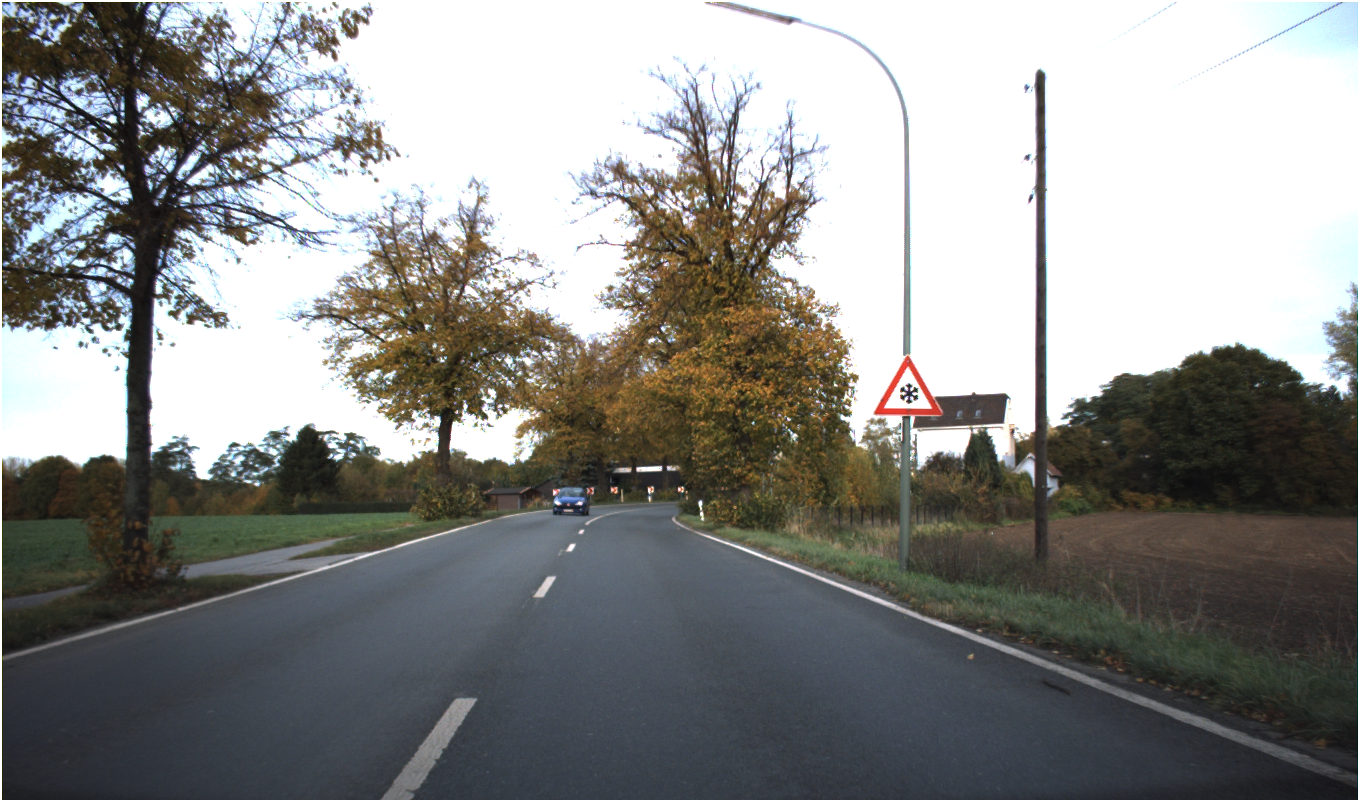
\includegraphics[scale=0.3]{sample_street}
            \caption{One of the images included in the GTSDB dataset}
        \end{figure}
    
        The GTSDB homepage can be found here: \url{https://benchmark.ini.rub.de/gtsdb_news.html}
        
        \subsection{You Only Look Once}
        
        You Only Look Once (YOLO) is a state-of-the-art real-time object detection system utilizing Darknet, an open-source neural network framework written with C and CUDA \cite{darknet13}. YOLO offers real-time neural network object detection that rivals other neural network frameworks Google and Facebook in accuracy and efficiency \cite{Bochkovskiy_2020}. The Darknet framework allows for researchers to utilize various YOLO versions for training on CPUs, GPUs, and on the cloud with Google Colab.  \\
        
        The Darknet framework can be found here: \url{https://github.com/AlexeyAB/darknet}
    
    \pagebreak
    \section{Training YOLO on GTSDB}
    
        \subsection{Specifications}
        
        This study, consisting of GTSDB data processing and two trials of YOLOv4 neural network training, was run on my personal PC. My computer runs Windows 10 with an Intel Core i7-9700K CPU with 8 cores, 16GB RAM, and an NVIDIA GeForce RTX 2070 Super GPU. 
        
        To run my study, I utilized the Python IDE Jetbrains PyCharm v2021.2 (Professional Edition), Microsoft Visual Studio Community 2019, OpenCV v4.5.3, CUDA v11.2, and CuDNN v8.2.1. 
        
        \subsection{Annotating}
        
            \subsubsection{Methodologies}
        
            The full GTSDB dataset was downloaded via the GTSDB homepage. This installation included not only the entire 900 image collection but also the ground truths for each image (Figure 2).
            
            \begin{figure}[h]
                \centering
                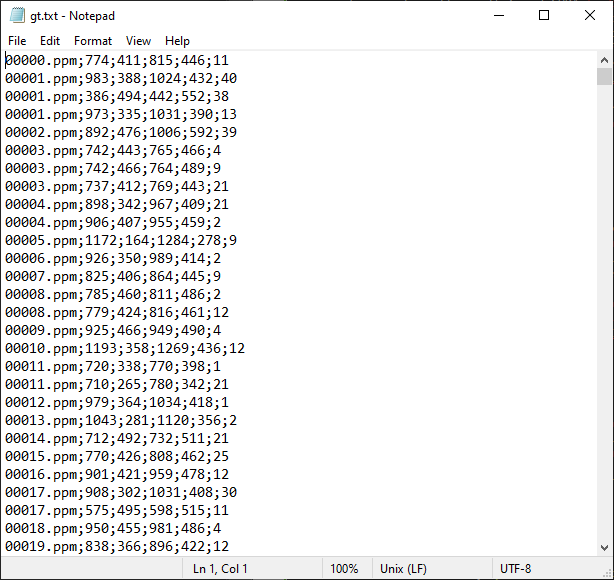
\includegraphics[scale=0.5]{ground_truths}
                \caption{The provided ground truths for each image in the GTSDB dataset}
            \end{figure}
        
            Each entry in the ground truth text file represents a detectable road sign and is formatted as such:
            
            \begin{center}
                \texttt{\textcolor{red}{00000.ppm;}\textcolor{blue}{774;411;815;446;}\textcolor{ForestGreen}{11}}
            \end{center}
        
            With \texttt{\textcolor{red}{00000.ppm}} representing the image, \texttt{\textcolor{blue}{774;411;815;446}} representing the bounding box of the ground truth of the road sign in the picture (leftCol; topRow; rightCol; bottomRow), and \texttt{\textcolor{ForestGreen}{11}} representing the class to which the road sign belongs (Figure 3). Thus,  \texttt{\textcolor{red}{00000.ppm;}\textcolor{blue}{774;411;815;446;}\textcolor{ForestGreen}{11}} can be interpreted as a "priority at next intersection" sign in image \texttt{00000.ppm} within the box 774;411;815;446.
            
            \begin{figure}[h!]
                \centering
                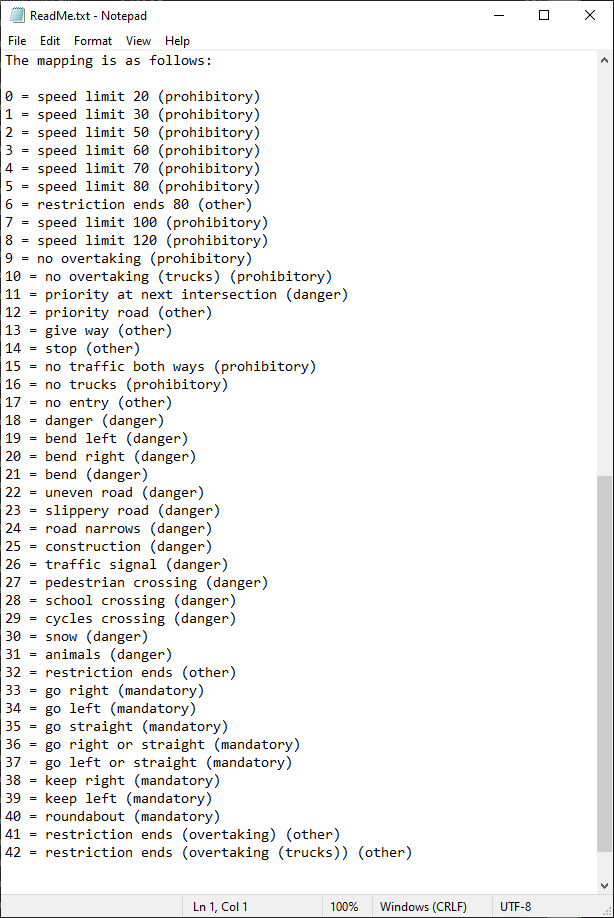
\includegraphics[scale=0.5]{original_classes}
                \caption{The provided classes of road signs found in the GTSDB dataset}
            \end{figure}
            \pagebreak
            
            The issue with this formatting of pre-annotated data was that Darknet recognizes a different syntax of image annotations as training and testing input. For example, for each image, there would exist a corresponding \texttt{.txt} file formatted as
            
            \begin{center}
                \textless class number\textgreater \; \textless x\_center\textgreater \; \textless y\_center\textgreater \; \textless width\textgreater \; \textless height\textgreater.
            \end{center}
        
            To format the annotated input images correctly, I utilized a tool called Datasets2Darknet, which runs a Python script to parse and convert several datasets, including GTSDB, into Darknet format labeled images. Datasets2Darknet randomly properly assigns images to training and testing sets depending on the given train-to-test ratio and reduces the original number of GTSDB classes (43) to a small number of generalized classes. A \texttt{train.txt} and \texttt{test.txt} file is created listing all of the images corresponding the training and testing sets. \\
            
            Datasets2Darknet can be found here: \url{https://github.com/angeligareta/Datasets2Darknet}
        
        \subsection{Neural Network Training, Trial 1}
        
            This first trial was an initial test of YOLOv4 without making any modifications. The purpose of including this run is to detail the improvements and adjustments I needed to make to obtain better results.
        
            \subsubsection{Methodologies}
            
            For my initial run of neural network training, I chose to allocate 90\% of the GTSDB dataset as training data and the remaining 10\% as testing. I utilized the Datasets2Darknet tool to allocate the GTSDB dataset into 10 classes, and the distribution of these images is shown in Figure 4. 
            
            \begin{figure}[h]
                \centering
                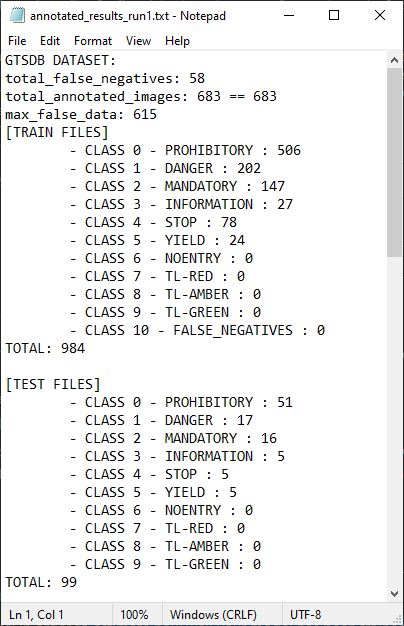
\includegraphics[scale=0.5]{run_1_annotated}
                \caption{The results of dataset allocation for trial 1}
            \end{figure}
        
            After configuring and building Darknet with OpenCV, CUDA, and CuDNN with Visual Studio, the newly formatted images and corresponding text files were then fed into the YOLOv4 algorithm for training on my GPU. 
        
            \subsubsection{Results}
            
            Training the GTSDB data for 20000 iterations (number of classes * 2000) took roughly 12 hours, allowing me to understand how YOLOv4 measured model reliability. 
            
            \begin{itemize}
                
                \item Intersection Over Union (IoU): the ratio of the area of the intersection of the ground truth annotated label box and the detected box to the union of the area between the two boxes; the closer to 1 the better, signifying accurate and precise detection of target objects. A threshold for IoU can be configured to determine whether a detection is labeled a true or false positive. 
                
                \begin{figure}[h]
                    \centering
                    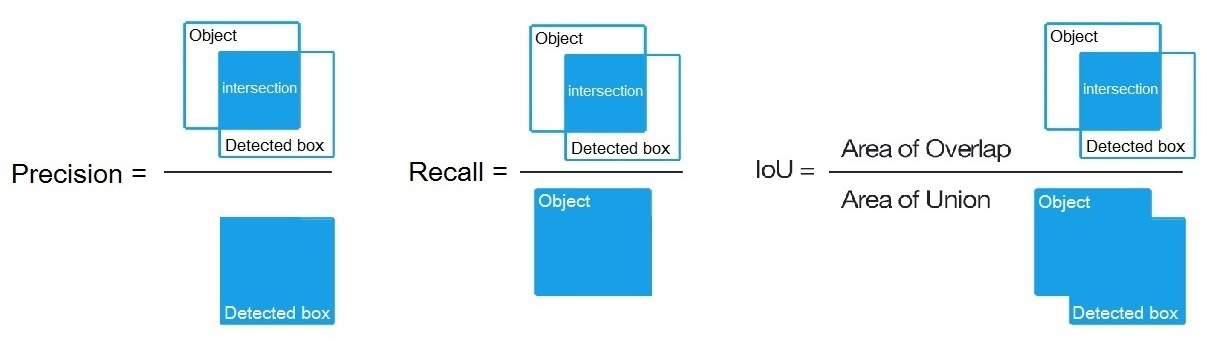
\includegraphics[scale=0.5]{iou}
                    \caption{Demonstration of the IoU metric}
                \end{figure}
            
                \item Mean Average Precision (mAP): the average of the area under the precision-recall curve for each class \cite{bochkovskiy2020yolov4, Yohanandan_2020}. Here, precision is defined as how accurate the model can correctly predict (percentage of predictions that are correct) and is calculated by
                
                \[\textit{Precision} = \frac{\text{True Positives}}{\text{True Positives} + \text{False Positives}}\]
                
                whereas recall measures how well the model can find all the positives, calculated as
                
                \[\textit{Recall} = \frac{\text{True Positives}}{\text{True Positives + False Negatives}}.\]
                
                Average precision is described as the area under the precision-recall curve for each class, making the mean average precision to be the the averages of average precisions \cite{Yohanandan_2020}. Generally, the higher the mAP value the better the model detects the target objects.
                
                \item F1 Score: a popular metric in determining model accuracy utilizing precision and recall. F1 score can be calculated as
                
                \[\textit{F1 Score} = 2 * \frac{\text{Precision} * \text{Recall}}{\text{Precision} + \text{Recall}}.\]
                
            \end{itemize}
        
            Upon evaluating the trained model on the test dataset, for a detection threshold of 0.25 and IoU threshold of 50\%,
            
            \begin{itemize}
                
                \item Precision = 0.98
                \item Recall = 0.86
                \item F1 Score = 0.92
                \item Average IoU = 90.21\%
                \item mAP@0.50 = 54.05\%
                
            \end{itemize}
        
            after 20000 iterations.
        
            Although the predictions my model makes is mostly correct, my model seems to fail at detecting objects, as observed in my high number of false negatives.
            
            \begin{figure}[h!]
                \centering
                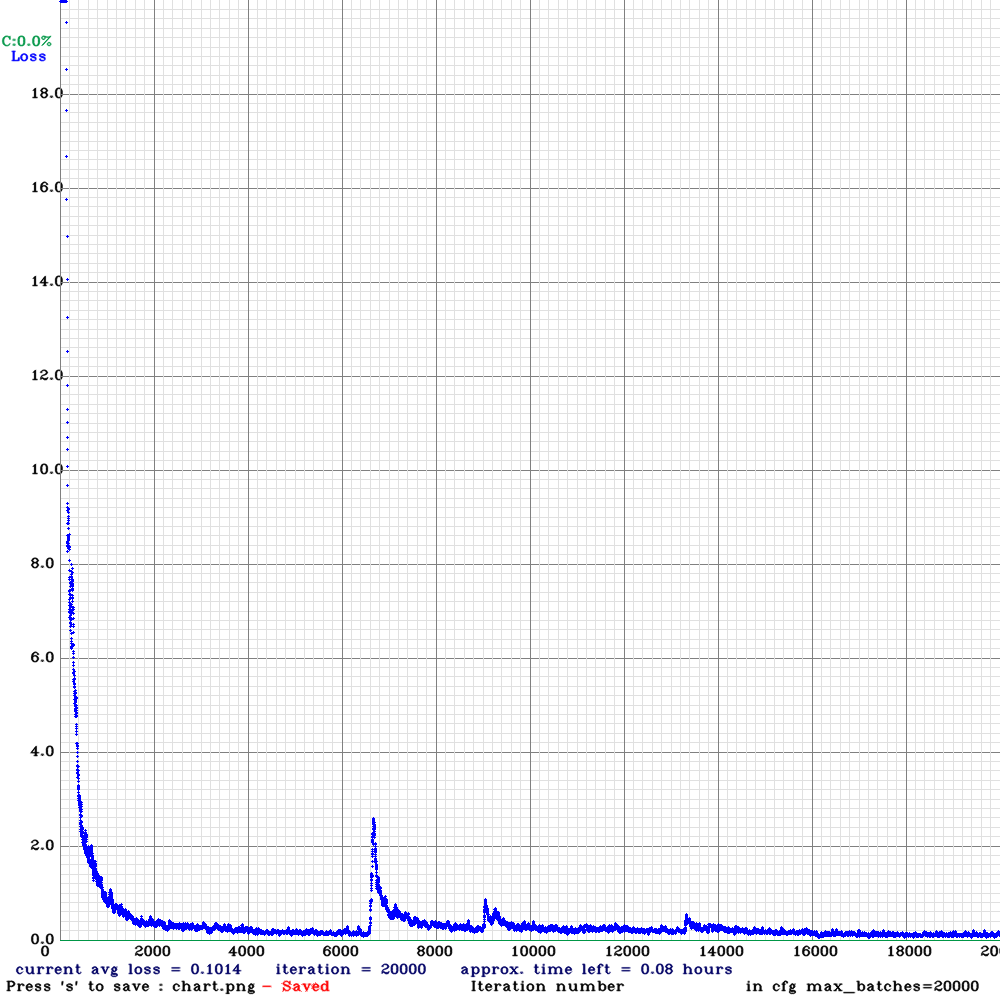
\includegraphics[scale=0.4]{gtsdb_trial1}
                \caption{Average loss during training YOLOv4 for trial 1}
            \end{figure}
            
            \pagebreak
            \subsubsection{Improvements to make}
            
            Upon review, I realized that the model had actually starting overfitting the training data, hence the large number of false negatives and thus low recall and low mAP. Going through my methodologies, I found the culprit to be my configuration of the Datasets2Darknet tool. I was utilizing classes that were not found in the GTSDB dataset but rather in the other similar datasets that Datasets2Darknet supports. In actuality, the \texttt{gtsdb\_parser.py} file in Datasets2Darknet listed only 6 generalized classes, omitting the "INFORMATION" and "TL-" categories found in my original method of GTSDB dataset allocation. Seeing that the number of batches (and thus number of iterations) was to be decided by multiplying the number of classes with 2000, the original configuration resulted in 20000 iterations when the correct number of batches should have been 6 * 2000 = 12000. These improvements would soon be made in the subsequent training of the neural network.
        
        \subsection{Neural Network Training, Trial 2}
        
            Taking my results from trial 1 into consideration, I changed my configuration of annotated data and kept my YOLO configuration the same, as I was confident that my issue with detection in trial 1 was overfitting due to accounting for unnecessary classes. 
        
            \subsubsection{Methodologies}
            
            I ran the GTSDB dataset through Datasets2Darknet once again, however this time cutting down the number of classes to the 6 necessary classes organized as per the \texttt{gtsdb\_parser.py} file. The number of batches then was cut to 12000, in hopes of preventing overfitting. Additionally, to further prevent overfitting, the train-to-test ratio was changed from 0.9 to 0.75, allowing for variation upon object detection. 
            
            \begin{figure}[h!]
                \centering
                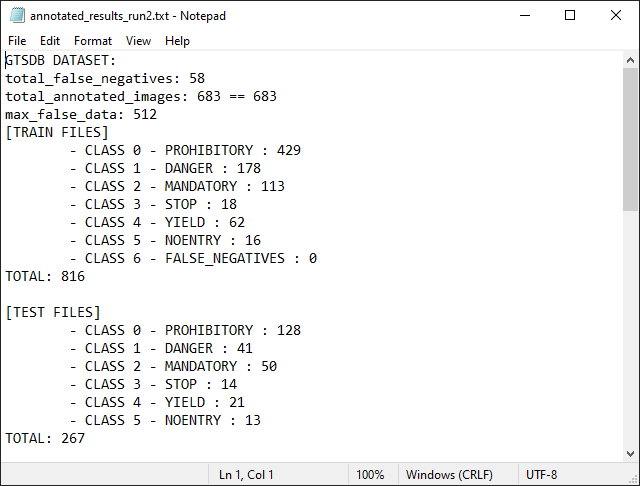
\includegraphics[scale=0.5]{run_2_annotated}
                \caption{The results of dataset allocation for trial 2}
            \end{figure}
        
            The newly allocated Darknet formatted dataset was then fed to YOLOv4 for training.
            
            \subsubsection{Results}
            
            Upon testing the trained YOLO model on my test dataset under the same detection and IoU thresholds, 
            
            \begin{itemize}
                
                \item Precision = 0.98
                \item Recall = 0.97
                \item F1 Score = 0.97
                \item Average IoU = 89.66\%
                \item mAP@0.50 = 95.10\%
                
            \end{itemize}
        
            after 12000 iterations. 
            
            I was impressed to see a significant increase in recall from the first trial. These results seem to confirm that my model from trial 1 was likely overfitted to the training data. My F1 score metric was greater this trial than it was in trial 1, meaning that this model was better at avoiding false positives while honoring true negatives. 
            
            \begin{figure}[h!]
                \centering
                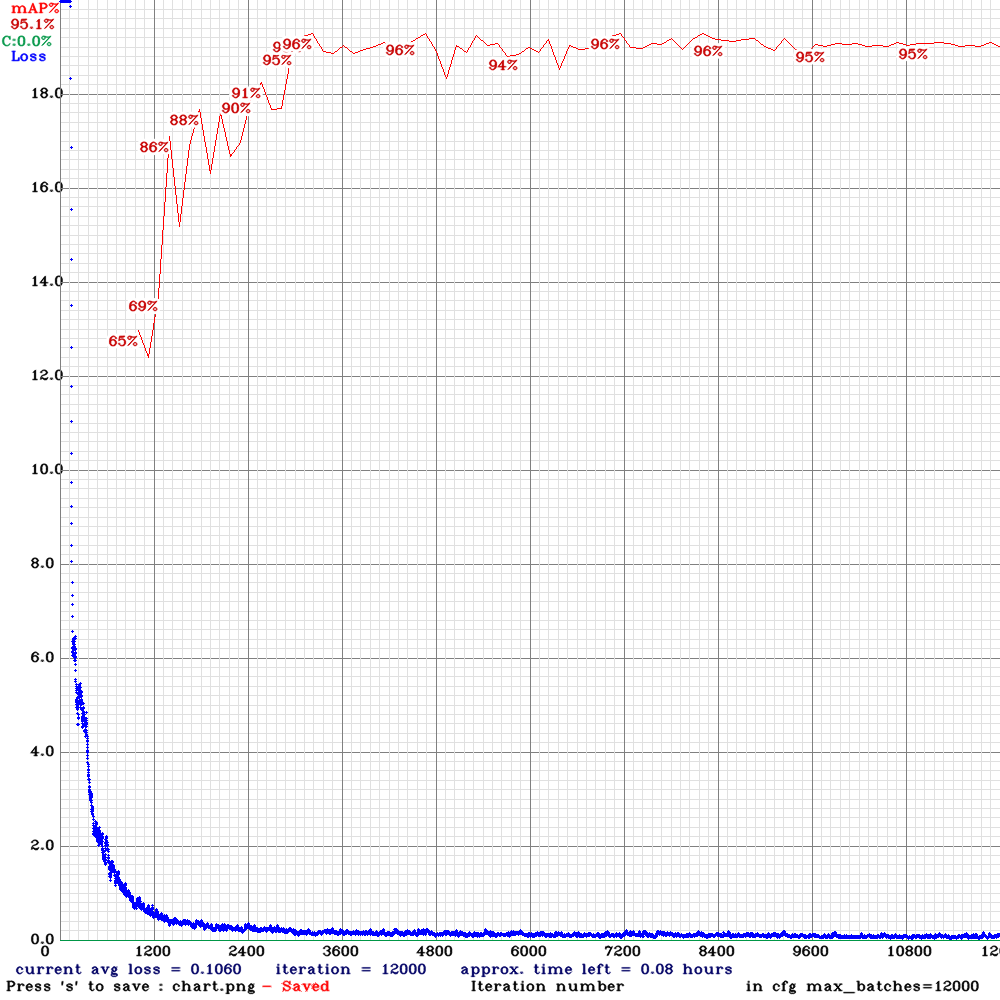
\includegraphics[scale=0.4]{gtsdb_trial2}
                \caption{Average loss during training YOLOv4 for trial 1, with mAP displayed in red}
            \end{figure}
            
            \subsubsection{Further Study}
            
            I would like to try training new models with altered hyperparameters and thresholds and observe the variations in model reliability. Modifying the number of iterations (as expected) made the model more reliable; given unlimited resources and unlimited time I am highly interested in determining the right parameter values to create an unrivaled state-of-the-art neural network. 
            
        \pagebreak
        \section{Reflection and Regards}
    
        \begin{enumerate}
            
            \item \textbf{YOLOv4 Hyperparameters}
            
            YOLOv4 is versatile and offers configurable hyperparameters (learning rate, epochs, optimization method, etc.) to fit most object detection and neural network needs. However, I decided to keep my hyperparameters consistent to the default configuration during both trials (outside of number of batches to fix overfitting and batch size with recommendation by users in the Darknet Discord channel). In the future I would like to explore the strength of certain hyperparameters and determine which ones I could alter to get my F1 score as possibly close to 1 as I can. 
            
            \item \textbf{Training Strategy}
            
            My training strategy was to let YOLOv4 run its iterations with help from the Datasets2Darknet repository. For training, following the guide on training custom datasets from the Darknet GitHub page was instrumental in learning how to configure YOLO to train my GTSDB dataset.
            
            \item \textbf{Detection Performance and Evaluation}
            
            I looked at model performance metrics such as the mean average precision value and F1 score to determine reliability of the trained models. The goal of neural network training is to maximize true positive and true negative counts while minimizing false positive and false negative counts. 
            
            \item \textbf{False Positive / False Negative Detection}
            
            My first trial exhibited a large number of false positives, meaning that my detector was sometimes not detecting road signs that should have been detected. I believed that this was a result of overfitting due to too many iterations. I trained YOLO again but this time reducing the number of classes and iterations by 40\%. Doing so yielded a higher reliability sporting a higher precision and recall.
            
            \item \textbf{Return to Data Annotating}
            
            After running trial 1, I did return to data annotating to fix my data allocation. 
            
            \item \textbf{Comparisons with State of the Art Object Detection}
            
            This study detailed and analyzed the training process and results for the GTSDB dataset, but only after processing all 43 original classes and conglomerating similar classes into 6 generalized Darknet classes. Although this method of classification exhibits great performance, I expect the reliability of this model to decrease significantly if all 43 original classes were trained, as the average number of images per class would then decrease significantly. Some modifications seen in similar implementations of YOLO on GTSDB were varying network resolution in the \texttt{.cfg} file, adding additional convolutional layers, and modifying the thresholds for IoU and detection. 
            
            \item \textbf{Main Challenges}
            
            My initial challenges was setting up the environment to run Darknet and YOLO. I spent a few days installing and building Darknet and its dependencies, but after running tests on pre-trained COCO models, I knew I had it up and running.
            
            Aside from environment setup, I did not have many other challenges training the network for the GTSDB dataset. Training this model was a learning experience every step of the way, and I am excited to pursue similar work in my career and research. 
            
            Lastly, I give my regards to Professor James Tsai and his graduate colleagues for assigning this interview activity. I am grateful for the chance to go beyond my comfort zone to show how quickly I can learn the fundamentals and utilize an unfamiliar framework to create a strongly reliable model.
            
        \end{enumerate}


    \pagebreak
    \bibliography{references}
    \bibliographystyle{acm}
    
    
    
\end{document}